\section{Création d'un point d'extension Eclipse}\label{section_build}

Pour introduire des fonctionnalités spécifiques à un modeleur, j'ai étudié la possibilité d'utiliser un point d'extension d'Eclipse pour gérer les parties spécifiques du modeleur.

\subsection{Principe}

Le principe d'un point d'extension est le suivant. 
Eclipse est une grosse boîte sur laquelle on peut se brancher, mais pas seulement (cf. figure \ref{extension_point}).
Il s'agit aussi de plusieurs centaines de petites boîtes reliées les unes aux autres qui peuvent être connectées par un plugin pour le modeleur Papyrus. 
Les plug-ins ou (bundles) fournissent des points d'extensions.

\subparagraph*{}
Il faut imaginer qu'il s'agit d'une multiprise de courant où l'on peut brancher autant de connexions (extensions) que ne peut supporter la multiprise (un point d'extension).

\begin{figure}[!ht]
\begin{center}
  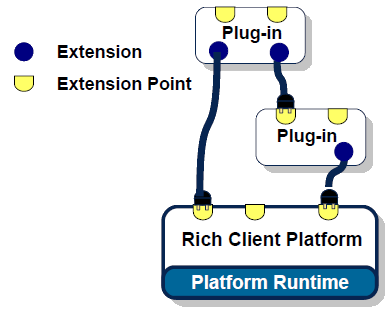
\includegraphics[scale=.5]{images/extension_point.png}
  \caption{Fonctionnement d'un point d'extension}
  \label{extension_point}
\end{center}
\end{figure}
\ \\
La première chose effectuée au moment du chargement d'un plugin, c'est les scans des metadata de tous les plugins, soit le fichier \texttt{plugin.xml}. 
Ceci n'étant effectué uniquement si les informations dans le cache d'Eclipse ne sont plus à jour, corrompues ou forcées (option -clean).

\subparagraph*{}
Si on exploite correctement les points d'extensions, il est possible de construire une interface graphique sans charger le plugin avec juste les metadata. 
Charger un plugin prend évidement de la mémoire et allonge le temps de démarrage d'Eclipse.

\subparagraph{Que se passe t'il lorsqu'un point d'extension est chargé ?}
Tout d'abord le fournisseur d'un point d'extension déclare celui-ci au registre d'extension.
Ensuite chaque plugin utilisant une extension s'identifie auprès du registre d'extension. Ces deux tâches sont automatiques, elles sont réalisées à partir du contenu des metadata (\texttt{MANIFEST.MF} et \texttt{plugin.xml}).

A partir de là, le fournisseur du point d'extension peut demander à instancier la classe déclarée par l'utilisateur du point d'extension (cf. diagramme de \ref{extension_point_sequence} p. \pageref{extension_point_sequence}).

\begin{figure}[!ht]
\begin{center}
  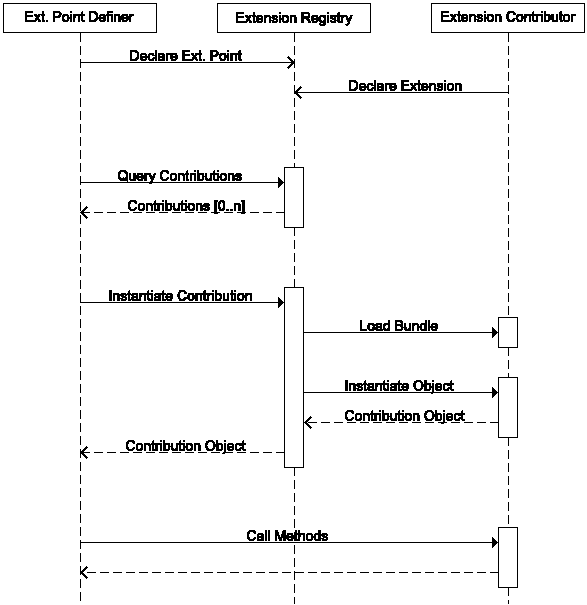
\includegraphics[scale=.7]{images/extension_sequense_diagram.png}
  \caption{Diagramme de séquence de l'enregistrement d'un point d'extension}
  \label{extension_point_sequence}
\end{center}
\end{figure}

\subparagraph{Précautions :}
Si un point d'extension est déclaré pour fournir une classe implémentant une interface I dans le plugin A. 
L'interface I doit être fournie par le plugin A déclarant le point d'extension.
Chaque plugin possède son propre environnement d'exécution\footnote{ClassLoader pour les programmeurs Java} (cf .\ref{OSGI} p.\pageref{OSGI}).
Ce qui signifie que la classe doit implémenter l'interface I du même environnement d'exécution (plugin A).
Même chose pour le type de retour des fonctions et ses paramètres, eux aussi doivent appartenir au même environnement d'exécution.

\subparagraph*{}
C'est a cette occasion que l'on utilise l'exportation de package dans le \texttt{MANIFEST.MF} via la propriété ``Export-Package''. Cette propriété permet de rendre visible par un autre plugin les classes contenues dans un package cible.

\subparagraph*{}
Avec ce mécanisme, il faut faire attention aux différents espaces de chargement des classes\footnote{ClassLoader}. Exemple : le plugin A propose le point d'extension \newline ``com.smartesting.core.extractor'' qui permet de définir une classe qui implémente l'interface  ``com.smartesting.extractor.Extractor'' via l'élément ``class''. Le plugin B utilise le point d'extension  ``com.smartesting.core.extractor'' avec comme classe \newline ``mon.plugin.extractor.MyExtractor''.

\subsection{Mise en \oe uvre}\label{subsection:MiseEnOeuvre}

Ce paragraphe explique le moyen de mise en \oe uvre d'un point d'extension pour gérer un extracteur de modèle spécifique au modeleur Papyrus. (A noter que les \ldots des exemples correspondent à un chemin de package).

\subsubsection{Etape 1 : Créer un point d'extension}

Il faut tout d'abord déclarer un point d'extension dans le plugin \texttt{Common Extractor} puisque tous les plugins d'export en dépendent.

Ensuite le point d'extension est définie dans le fichier \texttt{ModelExtractor.exsd}.
Puis on déclare dans le fichier \texttt{plugin.xml} le point d'extension :

\setlength\abovecaptionskip{0.25ex}
\setlength\belowcaptionskip{0.25ex}

\begin{figure}[H]
\centering
\begin{lstlisting}[language=XML]
<plugin>
	<extension-point id="ModelExtractor" 
		name="com.smartesting.eclipse.core"
	schema="schema/ModelExtractor.exsd"/>
</plugin>
\end{lstlisting}
\caption{Extrait du fichier \texttt{ModelExtractor.exsd} dans le plugin ``Common extractor''}
\end{figure}

Ensuite le fichier \texttt{Modelextractor.exsd} est configuré afin de permettre la déclaration de l'utilisation de l'extension comme ceci :
\begin{figure}[H]
\centering
\begin{lstlisting}[language=XML]
<extension point="com.smartesting.eclipse.core.ModelExtractor">
  <ModelExtractor
	  class="...PapyrusModelExtractor"/>
</extension>
\end{lstlisting}
\caption{Extrait du fichier \texttt{plugin.xml} du plugin ``Papyrus extractor''}
\end{figure}
Dans l'exemple précédent, l'attribut ``class'' permet de définir la classe qui permettra de rendre le service. 
Il a été choisi que la classe \texttt{PapyrusModelExtractor} devrait implémenter l'interface ``ModelExtractor''. 

\subsubsection{Etape 2 : Utiliser le point d'extension}

Pour utiliser les données du point d'extension, il faut passer par la plateforme Eclipse et interroger l'\texttt{ExtensionRegistry}\footnote{Platform.getExtensionRegistry()}. Grâce à ce service, nous pouvons récupérer l'instance de l'interface \texttt{ModelExtractor} qui sera \texttt{PapyrusModelExtractor}.

\subsubsection{Etape 3 : Exporter les classes dépendantes}

La dernière étape mais non des moindres, doit permettre de rendre visible depuis un autre plugin l'interface \texttt{ModelExtractor} dont \texttt{PapyrusModelExtractor}.
Pour cela, on ajoute la ligne suivante dans le fichier \texttt{MANIFEST.MF} du plugin ``Common extractor'' :
\begin{figure}[H]
\centering
\begin{verbatim}Export-Package: . . .ModelExtractor\end{verbatim}
\caption{Fichier \texttt{MANIFEST.MF} du plugin ``Common extractor''}
\end{figure}

\begin{figure}[!ht]
\begin{center}
  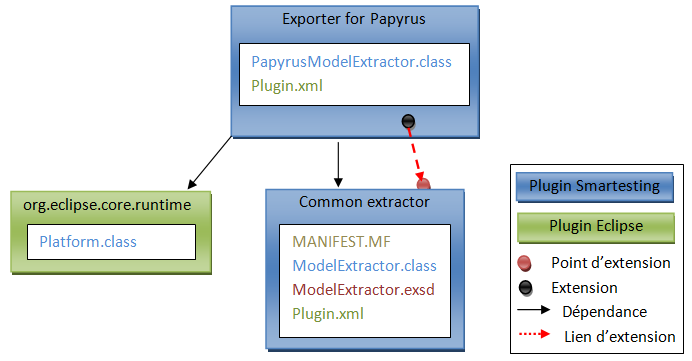
\includegraphics[scale=.5]{images/UsePapyrusExtensionPoint.png}
  \caption{Mise en \oe vre d'un point d'extension pour extraire le modèle UML}
  \label{figure:UsePapyrusExtensionPoint}
\end{center}
\end{figure}

La figure \ref{figure:UsePapyrusExtensionPoint} p.\pageref{figure:UsePapyrusExtensionPoint} montre l'infrastructure des plugins pour la mise en place du mécanisme de point d'extension.
\begin{description}
  \item [Le plugin ``Common extractor''] contient le fichier manifest dans lequel est déclaré visible la classe \texttt{ModelExtractor}.
Le fichier \texttt{ModelExtractor.exsd} contient la déclaration du point d'extension, son nom, sa structure XML. \texttt{Plugin.xml} contient la déclaration du fichier \texttt{ModelExtractor.exsd}.

\item [Le plugin ``Papyrus extractor''] contient un manifest contenant la dépendance avec ``Common extractor'', la classe spécifique d'extraction du modèle appelé \newline \texttt{PapyrusModelExtractor} et le fichier \texttt{plugin.xml} pour déclarer l'utilisation du point d'extension.
\end{description}

\subsection{Avantages /inconvénients}

La mise en place du mécanisme d'un point d'extension est simple à mettre en place et offre des résultats rapides.
Il faut éviter le piège sur le problème d'environnement d'exécution différent des plugins.

\subparagraph*{}
Il y a cependant, un problème lié à l'environnement d'Eclipse, qui utilise des variables globales comme ``Platform'' qui empêchent la réalisation de tests unitaires simples. 
La solution est d'abstraire la plateforme Eclipse pour pouvoir tester le mécanisme.
